\section{Results and evaluation} \label{sec:results}

This section describes tests and benchmarks performed on different datasets,
along with evaluation and discussion of the results.

\subsection{Overview of datasets and hardware used for testing}
\label{sec:overview_of_datasets}

A couple of different datasets will be used for testing and evaluating the
implementation of the distance metrics and clustering algorithms presented in
section \ref{sec:methods}. These datasets will be briefly presented in this
section.

\begin{description}
  \item[\texttt{SILVA}] \hfill \\
    The dataset \texttt{SILVA\_119\_SSURef\_tax\_silva.fasta} has a size of
    around 2.3 GB and contains \num{1583830} RNA sequences.

  \item[\texttt{RDP}] \hfill \\
    The dataset \texttt{RDP\_Pro\_Full.sort.fna} has a size of around 3.5 GB
    and contains \num{3019928} DNA sequences.
\end{description}

The datasets are in \texttt{FASTA} format, where each sequence consists of the
character ``>'' followed by a description and a newline followed by the
sequence. An example of this would be
\begin{verbatim}
    >Description
    ACGATGCTAGCTAGCTAGCTAGCTGCGCTGA...
    >Another description
    TTTTTTAGTCGATGGGTGCATTGATGAGTAG...
\end{verbatim}

Various statistics about the datasets are shown in Table \ref{tab:data_stats}.
The error ratio is the ratio between the number of ambiguous bases and the
number of regular DNA/RNA bases.

\begin{table}[H]
  \centering
  \begin{tabular}{c | c | c | c | c | c}
    Dataset        & Avg. len. & Min. len. & Max. len. & Median len. & Error ratio \\
    \hline\hline
    \texttt{SILVA} & \num{1415.46}  & \num{900} & \num{3845} & \num{1389} & 0.000156146 \\
    \texttt{RDP}   & \num{1044.19}  & \num{400} & \num{2922} & \num{1132} & 0.000798764 \\
  \end{tabular}
  \caption{Various information about the different datasets.}
  \label{tab:data_stats}
\end{table}

The hardware used for testing was a 64-bit Intel Core i5-2520M 2nd generation,
Sandy Bridge processor with a base frequency of 2.5 GHz and with 2 cores (4
hardware threads), and 16 GB RAM.


\subsection{Testing the distance metric on altered sequences}
\label{sec:altered_sequences}

Four different sets of highly similar sequences were constructed from an RNA
sequence from \texttt{SILVA} and this was used in the evaluation of the
distance metric.

One sequence was chosen, 10 copies of this sequences were made and to each of
these copies, a few alterations were made. A list of random indices in the
sequence was generated and in each of these indices in the sequence, a
substitution for a different, randomly chosen nucleotide was made.  This was
done twice, for different degrees of alteration, and the number of alterations
was equal to respectively 1\% and 2\% of the length of the sequence.

For the two other sets, the same number of alterations to individual
nucleotides were made, but in this case they were grouped into alterations of
substrings of length 5 (one such group being of length less than 5 if the
number of alterations was not a multiple of 5).

For illustration, Figure \ref{fig:alterations} shows an original sequence in
the first line, the single edits altered sequence in the second line and the
chunk altered sequence in the third line.

\newcommand{\tc}[1]{\textcolor{red}{#1}}
\begin{figure}[H]
  \centering
  \texttt{AAAAAAAAAAAAAAAAAAAAAAAAAAAAAA} \\
  \texttt{AA\tc{G}AAAA\tc{T}AA\tc{C}AA\tc{T}A\tc{C}A\tc{G}AAA\tc{C}AA\tc{T}AAAAA} \\
  \texttt{AAAAA\tc{TCGT}AAAAAAAAAA\tc{TTGG}AAAAAAA}
  \caption{Two types of alterations to sequences: the original sequence in the
    first line, single edit alterations in the second line and chunks of edits
    in the third line.}
  \label{fig:alterations}
\end{figure}

The $k$-mer based distance metric, presented in section
\ref{sec:kmer_distance}, is expected to be more sensitive to a number of
individual changes than to the same number of changes made in chunks. This test
serves to confirm this expectation and to give an insight into the change in
$k$-mer distance when performing a controlled number of edits.

The similarities between the original sequence from \texttt{SILVA} and the 10
altered sequences, for the four different types of alterations, are shown in
Table \ref{tab:altered_seqs_similarities}.

\begin{table}[H]
  \centering
  \begin{tabular}{c|c||c|c}
    \multicolumn{2}{c||}{single edits}  & \multicolumn{2}{c}{chunk edits} \\
    \hline\hline
    1\%   &   2\%                   &   1\%   &   2\% \\
    \hline
    0.944   & 0.889                     & 0.980     & 0.960 \\
    0.947   & 0.887                     & 0.979     & 0.960 \\
    0.944   & 0.893                     & 0.979     & 0.960 \\
    0.941   & 0.902                     & 0.979     & 0.961 \\
    0.944   & 0.894                     & 0.979     & 0.958 \\
    0.947   & 0.894                     & 0.979     & 0.958 \\
    0.941   & 0.895                     & 0.982     & 0.958 \\
    0.945   & 0.891                     & 0.979     & 0.961 \\
    0.945   & 0.889                     & 0.979     & 0.958 \\
    0.946   & 0.897                     & 0.981     & 0.958
  \end{tabular}
  \caption{Similarity measures, using $k=6$, for 1\% and 2\% single edits,
    respectively, and 1\% and 2\% chunk edits, respectively, to 10 copies of a
    single sequence.}
  \label{tab:altered_seqs_similarities}
\end{table}

As expected, the single edits result in a lower similarity than the
corresponding chunk edits. This is because five individual changes will affect
the count of up to $5 \cdot k$ $k$-mers, while five changes in sequence will
only affect up to $4+k$ $k$-mers.


\subsection{Comparing \textsc{K-Dist} with the Levenshtein distance metric}
\label{sec:kdist_vs_levenshtein}

This section compares the implementation of the \textsc{K-Dist} distance
metric with the implementation of the bottom-up dynamic programming algorithm
for the Levenshtein distance metric (Algorithm \ref{alg:levenshtein} in
appendix \ref{app:levenshtein_algorithm}).

The data in Table \ref{tab:levenshtein_vs_kdist_performance} shows how many
comparisons per second the implementation of Levenshtein and the implementation
of \textsc{K-Dist} can afford. This is shown for various values for the $k$
parameter. The tests were performed on the \texttt{SILVA} dataset.

\begin{table}[H]
  \centering
  \begin{tabular}{ c | r }
    Distance metric implementation  & Comparisons/second    \\
    \hline \hline
    Levenshtein (DP)                & $\approx \num{195}$   \\ \hline
    \textsc{K-Dist}, $k=4$          & $\approx \num{91500}$ \\ \hline
    \textsc{K-Dist}, $k=5$          & $\approx \num{91000}$ \\ \hline
    \textsc{K-Dist}, $k=6$          & $\approx \num{89000}$ \\ \hline
    \textsc{K-Dist}, $k=7$          & $\approx \num{72500}$ \\ \hline
    \textsc{K-Dist}, $k=8$          & $\approx \num{46000}$ \\
  \end{tabular}
  \caption{Performance comparison between the bottom-up, dynamic programming
    Levenshtein implementation and the \textsc{K-Dist} implementation with
    different values for the $k$ parameter. Tested on the \texttt{SILVA}
    dataset.}
  \label{tab:levenshtein_vs_kdist_performance}
\end{table}

The \textsc{K-Dist} implementation with $k=4$ is more than 460 times faster
than the Levenshtein implementation, but becomes slower with increasing values
for $k$, with the \textsc{K-Dist} implementation being around 235 times faster
for $k=8$.

As mentioned in section \ref{sec:edit_distance}, the running time of the
presented Levenshtein algorithm is near quadratic in the lengths of the
strings, while the running time of the \textsc{K-Dist} algorithm is
$\Theta(\max{(\abs{s},\abs{t})}-k)$, where $s$ and $t$ are the sequences being
compared and $k$ is the value for the parameter $k$. This was analyzed in
section \ref{sec:k-dist_analysis}. So \textsc{K-Dist} will always be faster
than the presented algorithm for Levenshtein for long enough sequences and as
shown above in Table \ref{tab:levenshtein_vs_kdist_performance}, that is indeed
the case for the sequences this project is concerned with.

Scatter plots of \textsc{K-Dist} similarities and the corresponding Levenshtein
similarities for parameters $k=5$ and $k=8$ are shown in Figure
\ref{fig:k-dist_lev_similarity_k5} and Figure
\ref{fig:k-dist_lev_similarity_k8}, respectively. These similarity measures
were obtained by comparing the 500 first sequences from \texttt{SILVA} with
each other.

\begin{wrapfigure}{l}{0.55\textwidth}
  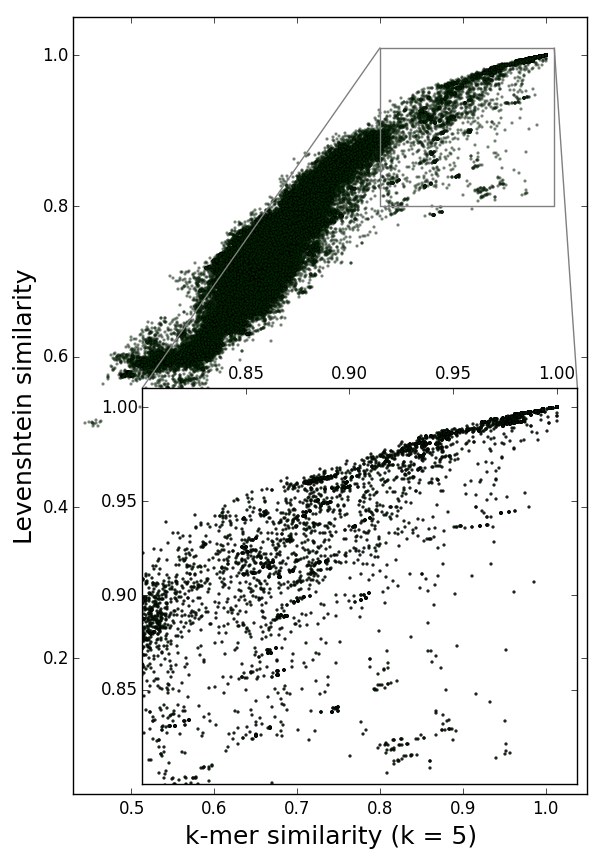
\includegraphics[width=0.55\textwidth]{graphics/Levenshtein_K-Dist_k5.png}
  \caption{Scatter plot comparison of similarity measures for Levenshtein and
    \textsc{K-Dist} with $k=5$ on the first 500 sequences of \texttt{SILVA}.}
  \label{fig:k-dist_lev_similarity_k5}
\end{wrapfigure}

Since the Levenshtein distance does not produce values between 0 and 1, a
similarity ratio similar to the one used in \textsc{K-Dist} and expressed in
equation (\ref{eq:Manhattan_similarity}) was used. Specifically, the ratio
between the Levenshtein distance and the maximum possible distance subtracted
from one. The maximum possible Levenshtein distance is equal to the length of
the longer sequence.

As seen in the figures, there is a monotonically increasing relationship
between the two similarity metrics. Additionally, the Levenshtein similarities
barely get below 0.5, while the interval of the \textsc{K-Dist} similarities is
around $[0.4,1.0]$ for $k=5$ and $[0,1]$ for $k=8$. This is likely because the
number of different 8-mers is much greater than the number of different 5-mers,
so it is less likely that two $k$-mers are the same. That will result in a
greater distance and hence a lower similarity.

Since \textsc{K-Dist} is not very sensitive to transpositions, but Levenshtein
is, there will be some measures which are relatively lower for Levenshtein than
for \textsc{K-Dist}. The ``width'' of the points in Figure
\ref{fig:k-dist_lev_similarity_k5} and \ref{fig:k-dist_lev_similarity_k8} can
partly be attributed to the difference in characteristic between the two
distance metrics. Additionally, the Levenshtein metric does not use a window
like K-Dist does and this will also contribute to some variance in the
similarity measures.


The subplots, i.e. the inner boxes, in Figure
\ref{fig:k-dist_lev_similarity_k5} and \ref{fig:k-dist_lev_similarity_k8},
shows a zoomed in view of the scatter plots in the interval $[0.8,1.0]$ on both
axes. The most interesting Levenshtein similarities are those above or equal to
$0.95$. These points lie fairly high for the corresponding \textsc{K-Dist}
similarity, for the most part, i.e. the majority of the comparisons that give a
Levenshtein similarity of $0.95$ also gives a \textsc{K-Dist} similarity of
$0.85$ or above.

\begin{figure}[h!]
  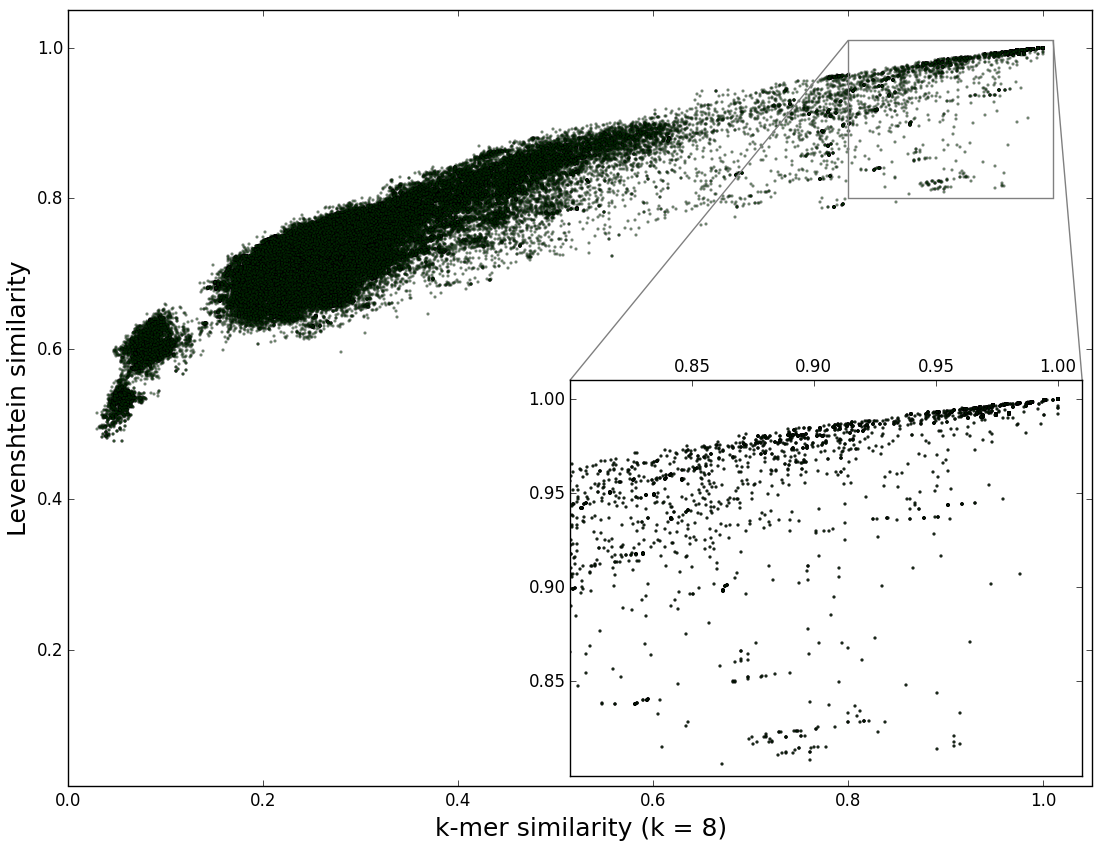
\includegraphics[width=1.0\textwidth]{graphics/Levenshtein_K-Dist_k8.png}
  \caption{Scatter plot comparison of similarity measures for Levenshtein and
    \textsc{K-Dist} with $k=8$ on the first 500 sequences of \texttt{SILVA}.}
  \label{fig:k-dist_lev_similarity_k8}
\end{figure}


\subsection{Evaluating \textsc{K-Clust} on a synthetic dataset}
\label{sec:synth_dataset}

A synthetic dataset was constructed for evaluating the \textsc{K-Clust}
algorithm's ability to find the right clusters in a dataset with a clearly
correct, expected clustering result.

A set of $380$ sequences with mutual \textsc{K-Dist} similarities of at most
$0.6$, using parameter $k=5$, was extracted from \texttt{SILVA}. For each of
these sequences, $999$ copies were made and chunks of changes were made to
these as described in section \ref{sec:altered_sequences}, corresponding to
$2$\% of the characters of each sequence. This yields a set of \num{380000}
sequences with $380$ expected clusters, which each should contain sequences
with similarities of approximately $0.92$ since all sequences are changed and a
$2$\% change to a sequence gives an average similarity from the original
sequence of around $0.96$, cf. section \ref{sec:altered_sequences}.

The sequences expected to be in the same cluster was given the same description
in the \texttt{FASTA} file, i.e. the same text string after ``>'', to make it
easy to evaluate the result from the clustering. Furthermore, the sequences
were placed in random order before running \texttt{klust} on the data.

The synthetic dataset was made fairly large, both in number of sequences and in
number of expected clusters, to be able to properly test the clustering
algorithm's ability to search for the correct centroid and not stop the search
prematurely which would result in a new cluster being created and a different
clustering result than the expected one.

As hoped, running \texttt{klust} on the constructed dataset, with parameters
$k=5$, $id=0.85$ and $max\_rejects=8$ gives a clustering output consisting of
$380$ clusters with 1000 sequences in each (including the centroid). The
terminal output from the program is shown in Figure
\ref{fig:synth_silva_output} in appendix \ref{app:synth_dataset} and an excerpt
from the clustering output file created by the program is shown in Figure
\ref{fig:synth_silva_clustering} in the same appendix. This shows that the
sequences in each cluster have the same description line, i.e. they were
constructed to be similar and should indeed be in the same cluster. The result
was equally correct when clustering with a threshold parameter of $0.89$, but
the results start containing a few errors when clustering with a threshold of
$0.9$ or above. In the specific test, and the specific, random order of the
sequences, the clustering result yielded $386$ clusters for $id=0.9$, an
average cluster size of $984.46$ and a minimum cluster size of $33$.

The same test was performed with \texttt{USEARCH}, though it requires the input
to be sorted. This actually produces $382$ clusters at both $id=0.95$ and $0.9$
where $0.9$ is quite low in \texttt{USEARCH}. At $id=0.87$ it makes $380$
clusters, but with a minimum cluster size of $38$. This means it does not find
the intended clusters in the synthetic dataset. The reason it does not find the
intended clusters can most likely be attributed to how it searches for
potential centroids.

This test provides some evidence that \textsc{K-Clust} is able to successfully
cluster a dataset of a fairly realistic size. Since the similarities are known
a priori and the cluster sequences are constructed to be of a similarity around
$0.92$ on $k=5$, this is not a test of the \textsc{K-Dist} distance metric.

\subsubsection{Multidimensional scaling of the synthetic dataset}
\label{sec:mds_synth}

\emph{Multidimensional scaling} (MDS) of the sequences in the synthetic dataset
was used to visualize and further evaluate the clustering result from the
previous section (section \ref{sec:synth_dataset}). Multidimensional scaling is
used to visualize the distances between objects in a high dimensional space in
two dimensions, i.e. it takes all distances between points in a high
dimensional space and tries to reflect these pairwise distances in two
dimensions.

The technique used for dimensionality reduction was \emph{t-distributed
Stochastic Neighbor Embedding} (t-SNE)~\cite{maaten}. This was done using
\texttt{Python} with \texttt{matplotlib} and \texttt{scikit-learn}. Sequences
expected to be in the same cluster were given the same color and thus the MDS
is expected to give a visualization of separate clusters of points of the same
color. Centroids were given a circle marker with the same color as the
sequences in the cluster they represent, and all other sequences were gives a
``+'' marker.

A subset of the synthetic set described in section \ref{sec:synth_dataset} was
used for the MDS, because the scatter plot easily becomes too densely
populated and because the computation is too expensive for \num{380000}
sequences. A set of $400$ sequences, consisting of $40$ expected clusters with
$10$ sequences in each, was used for the visualization shown in Figure
\ref{fig:mds_synth}. MDS is performed based on \textsc{K-Dist} and the
coloring is based on \textsc{K-Clust}, which is also based on \textsc{K-Dist}.
However, the MDS is based on the set of all distances while \textsc{K-Clust}
is heuristic, so the purpose is to test how good \textsc{K-Clust} is at
identifying the clusters that appear. Note that the MDS is used on the actual
distances and not the similarities.

\begin{figure}[h!]
  \def\svgwidth{\columnwidth}
  \import{graphics/}{MDS_Synthetic.pdf_tex}
  \caption{Multidimensional scaling using t-SNE of the 400 sequences and
    40 expected clusters from the synthetic dataset described in section
    \ref{sec:synth_dataset}. The distances are calculated using
    \textsc{K-Dist}. The clustering result from \texttt{klust} with $k=5$,
    $id=0.85$ and $max\_rejects=8$ is used to color different clusters with
    different colors. Centroids are marked with a circle and non-centroid
    sequences with a ``+''.}
  \label{fig:mds_synth}
\end{figure}

The result from \texttt{klust} on the synthetic dataset was correct and
completely as it was constructed to be. Similarly, the MDS in figure
\ref{fig:mds_synth} shows a very clear set of clusters of points, of distinct
colors and a single centroid for each cluster. There are only small errors such
as single sequences lying a bit away from their respective clusters and very
closely positioned clusters. However, this might easily have to do with the
actual MDS visualization of the data, since MDS does not provide a perfect
two-dimensional version of the high-dimensional distances.

Figure \ref{fig:mds_synth_lev} shows the same clustering result as in Figure
\ref{fig:mds_synth}, i.e. the same coloring and marking, but with the distances
for the MDS calculated using Levenshtein. This provides some more insight
into the relationship between \textsc{K-Dist} and Levenshtein, and helps to
verify the suitability of \textsc{K-Dist} as an approximation for sequence
similarity.

\begin{figure}[h!]
  \centering
  \def\svgwidth{\columnwidth}
  \import{graphics/}{MDS_Levenshtein.pdf_tex}
  \caption{Multidimensional scaling using t-SNE of the 400 sequences and 40
    expected clusters from the synthetic dataset using Levenshtein distance.
    The clustering result from \texttt{klust} with $k=5$, $id=0.85$ and
    $max\_rejects=8$ is used to color different clusters with different
    colors. Centroids are marked with a circle and non-centroid sequences
    with a ``+''.}
  \label{fig:mds_synth_lev}
\end{figure}

Once again, the results look very clear and as hoped, but there does seem to be
a little more overlap in the clusters, although this might again be partly
attributed to the imperfection of MDS. In any case, the clusters are also very
apparent when using the Levenshtein distance measure and this indicates that
the $k$-mer based \textsc{K-Dist} functions properly as an approximation of
distance. Specifically, the colors are not mixed up so it is not the case that
one distance metric gives a very low distance while the other gives a very
high distance, and vice versa, for some sequences.


\subsection{Evaluating \textsc{K-Clust} on real data using MDS}
\label{sec:mds_real_data}

The \textsc{K-Clust} algorithm was also tested on real data, specifically the
first 500 sequences of the \texttt{SILVA} dataset, using MDS to visualize the
sequence similarities and the clustering result, as described in section
\ref{sec:mds_synth}.


The clustering result from \texttt{klust} on \texttt{SILVA} consists of
clusters of very different sizes and a large number of singleton clusters, i.e.
clusters containing only the centroid sequence. This means that this data will
be harder to visualize nicely with MDS, since the sequences will not be as
clearly partitioned into a few clusters of the same size. However, it should at
least be possible to identify the sequences of large clusters, i.e. sequences
marked with the same color, and observe whether they are indeed close to each
other in the MDS.

Figure \ref{fig:mds_silva_sort_incr} shows MDS of the first 500 sequences from
\texttt{SILVA}, with the sequences sorted by increasing length before
clustering with \texttt{klust}. Figure \ref{fig:mds_silva} in appendix
\ref{app:mds_silva} shows the same results, but where sequences were not sorted
and sorted by decreasing length, respectively.

\begin{figure}[h!]
  \centering
  \def\svgwidth{\columnwidth}
  \import{graphics/}{graphics/MDS_Silva_incr.pdf_tex}
  \caption{MDS using t-SNE of the first 500 sequences from \texttt{SILVA} with
    the clustering result from \texttt{klust}, using parameters $k=5$,
    $id=0.85$ and $max\_rejects=8$, used to color different clusters with
    different colors. Centroids are marked with a circle. Sequences were sorted
    by increasing length before clustering.}
  \label{fig:mds_silva_sort_incr}
\end{figure}

The figures show a few apparent clusters, but as expected they also show a
large number of smaller clusters and singleton clusters. For the example in
Figure \ref{fig:mds_silva_sort_incr}, when running \texttt{klust} with
parameters $k=5$, $id=0.85$, $max\_rejects=8$ and sorting by increasing length,
the number of resulting clusters were $157$ with a maximum cluster size of $43$
and an average size of approximately \num{3.18}. Furthermore, the result
contained $89$ singleton clusters.

As expected, the sequences that were assigned to the same cluster are generally
close to each other in the MDS. The large number of singleton clusters and
small clusters are especially apparent in the centers of the figures and in the
lower left parts of the figures. Since the number of clusters is so high, it is
likely that the MDS causes the sequences to be more crammed together and appear
more dense than if the number of clusters had been lower.


\subsection{Evaluation of centroid search in \texttt{klust}}
\label{sec:evaluation_centroid_search}

A great part of efficient, greedy clustering lies in the task of locating
potentially matching centroids for a sequence. To evaluate this, \texttt{klust}
was run on a number of sequences from the dataset \texttt{SILVA} and various
information was extracted: how many times an actual comparison was made and did
not match; how often a comparison was not made, but it would have matched; how
often it performed a comparison against how often it did not and how often it
reached the $max\_rejects$ parameter. Table \ref{tab:centroid_search_data} show
this data represented as ratios. The program was run with parameters $k=5$,
$id=0.85$, $max\_rejects=8$ and sequences were sorted by increasing length.

\begin{table}[H]
  \centering
  \begin{tabular}{c||l|l}
  Count                                                    & \multicolumn{1}{c|}{\num{10000}} & \multicolumn{1}{c}{\num{100000}} \\
  \hline\hline
  Reject ratio ($\sfrac{rejects}{tries}$)                  & 0.00231                          & 0.00872                          \\
  \hline
  False negative ratio ($\sfrac{false\_negatives}{total}$) & 0.00048                          & 0.00013                          \\
  \hline
  Try ratio ($\sfrac{tries}{total}$)                       & 0.00377                          & 0.00112                          \\
  \hline
  Reached $max\_rejects$                                   & 0                                & 4                                \\
  \end{tabular}
  \caption{Data on the first \num{10000} and \num{100000} sequences of
  \texttt{SILVA} showing: reject ratio, i.e. the number of failed comparisons
  divided by the total number of comparisons (not including links); false
  negative ratio, i.e. the ratio between the number of times a sequence was not
  compared to a centroid but would have matched it and the total number of
  iterations over centroids; try ratio, i.e. the ratio between the number of
  times the intersection criterion was passed and the total number of
  iterations over centroids; and reached $max\_rejects$, i.e. how many times a
  query sequence was dismissed because it was rejected too many times.}
  \label{tab:centroid_search_data}
\end{table}

There are very few rejects in both cases, which means the intersection
criterion is actually a very accurate representation of sequence similarity.
When clustering \num{100000} sequences, the reject ratio increases. This should
not be seen as a drawback for the clustering quality. On the contrary, it means
it performs more comparisons and as a result, the number of false negatives
fall. The only loss, besides making a couple of additional compares, is that it
can reject the same sequence too many times ($max\_rejects$) and make the
sequence a centroid without comparing it to the remaining centroids. If this
situation occurs, it is likely because a sequence has many distinct $k$-mers
and thus often passes the intersection criterion. Such a sequence will often
not match a centroid, and while it might match some centroid, without a
$max\_rejects$ parameter it can essentially compare to all centroids.

The try ratio, how often it succeeds in the intersection criterion, is quite
low and even falls when clustering more sequences. When clustering \num{100000}
sequences it will only make a comparison every $1$ in $900$ times. Even though
\textsc{K-Clust} almost only makes comparisons when they will be successful
anyway, it still iterates all the way through the list of centroids, when
neither a match is found nor $max\_rejects$ is reached, and calculates the
$k$-mer intersections with every centroid.  Since it already chooses to perform
the comparisons with very little error (small reject and false negative ratios)
the only way to make the clustering faster is to find the right centroids
faster. The purpose of a link is to improve this search (cf. section
\ref{sec:k-clust_algorithm}).


\subsection{Evaluating \texttt{klust} on real data and comparing with
            \texttt{USEARCH}}
\label{sec:evaluating_klust_real_data}

To test the performance of the program and evaluate the clustering results,
\texttt{klust} was run with different parameters and settings. The table in
appendix \ref{app:klust_data_parameters} shows output data from running
\texttt{klust} on the first \num{100000} sequences from \texttt{SILVA} with
different parameters. Sorting by increasing length is on average $21.65\%$
faster and never slower than when not sorting. It is also on average $42.63\%$
faster and never slower than when sorting by decreasing length. Furthermore,
sorting by increasing length has $8.77\%$ fewer clusters on average and never
more clusters than when not sorting. It has $25.07\%$ fewer clusters on average
and never more clusters than when sorting by decreasing length. This
observation, along with the positive results from testing on the synthetic
dataset and centroid search evaluation, shows that sorting by increasing
length is always preferable.

Generally higher $k$'s are also expected to produce more clusters, since the
comparison punishes mismatches more than lower $k$'s as discussed in section
\ref{sec:altered_sequences}. The higher $k$'s also make the program a lot
slower. Section \ref{sec:synth_dataset} and the multidimensional scaling plots
in Figure \ref{fig:mds_synth} and Figure \ref{fig:mds_silva_sort_incr} shows
that $k=5$ is a good choice in terms of sensitivity. Another interesting choice
is $k=6$, since it performs almost the same number of comparisons per second
(cf.  Table \ref{tab:levenshtein_vs_kdist_performance} in section
\ref{sec:kdist_vs_levenshtein}). These results give the incentive to further
study $k=5$ and $k=6$, when sorting by increasing length. The reason lower
values of $k$ are not investigated is because the number of distinct $k$-mers
is too low, so the interval the similarities will typically fall in will lay
quite high (see section \ref{sec:kdist_vs_levenshtein}). This could make for
``lucky'' coincidences, where $k=5$ is better at preventing them. Based on the
results in \ref{app:performance_results_full_SILVA}, setting $k$ to less than
$5$ does not seem to reduce the time it takes to cluster by a lot, so risking
that lucky coincidences happen more frequently is not worth the minor boost in
speed.

The table in appendix \ref{app:performance_results_full_SILVA} shows data
from \texttt{klust} using either \textsc{K-Clust} or \textsc{Simple-Clust} and
\texttt{USEARCH}. The programs have been run with different parameters on the
entire \texttt{SILVA} dataset. Table \ref{tab:full_silva_main_results} shows
the most important results found in the appendix.

\begin{table}[H]
  \footnotesize
  \begin{adjustbox}{center}
  \begin{tabular}{c|r|r|r|lr|l}
  \multirow{2}{*}{}
  Clustering & \multicolumn{1}{c|}{Time} & \multicolumn{1}{c|}{Throughput} & \multicolumn{1}{c|}{Clusters} & \multicolumn{2}{c|}{Cluster sizes}& \multicolumn{1}{c}{Max} \\
  algorithm & \multicolumn{1}{c|}{(sec.)} & \multicolumn{1}{c|}{(seqs./sec.)} & & & & \multicolumn{1}{c}{memory} \\
  \hline \hline
  \multirow{3}{*}
  {}\textsc{Simple-Clust}, & & & & Max. & - & \\
  $k=6, id=0.85, m=32,$    & \num{931.5} & \num{1700.34} & \num{1018140} & Avg. & $1.56$ & $\approx\num{1013}$ MB \\
  no sort                  & & & & Min. & \num{1} & \\
  \hline
  \multirow{3}{*}
  {}\textsc{K-Clust},  & & & & Max. & \num{57885} & \\
  $k=5, id=0.85, m=8,$ & \num{1144.6} & \num{1383.81} & \num{98354} & Avg. & $16.10$ & $\approx\num{1013}$ MB \\
  incr. sort           & & & & Min. & \num{1} & \\
  \hline
  \multirow{3}{*}
  {}\textsc{K-Clust},  & & & & Max. & \num{71407} & \\
  $k=5, id=0.90, m=8,$ & \num{2578.9} & \num{614.16} & \num{159812} & Avg. & $9.91$ & $\approx\num{1021}$ MB\\
  incr. sort           & & & & Min. & \num{1} & \\
  \hline
  \multirow{3}{*}
  {}\textsc{K-Clust},  & & & & Max. & \num{79599} & \\
  $k=6, id=0.85, m=8,$ & \num{1812.0} & \num{874.07} & \num{127711} & Avg. & $12.40$ & $\approx\num{1012}$ MB\\
  incr. sort           & & & & Min. & \num{1} & \\
  \hline
  \multirow{3}{*}
  {}\textsc{K-Clust},  & & & & Max. & \num{49479} & \\
  $k=6, id=0.90, m=8,$ & \num{3450.6} & \num{459.00} & \num{191361} & Avg. & $8.28$ & $\approx\num{1039}$ MB\\
  incr. sort           & & & & Min. & \num{1} & \\
  \hline
  \multirow{3}{*}
  {}\texttt{USEARCH},        & & & & Max. & \num{83904} & \\
  $id=0.95,$ decr. sort      & \num{1719.0} & \num{920.30} & \num{117205} & Avg. & $13.50$ & $\approx\num{1126}$ MB \\
  \texttt{-cluster\_smallmem} & & & & Min. & \num{1} & \\
  \hline
  \multirow{3}{*}
  {}\texttt{USEARCH},        & & & & Max. & \num{59820} & \\
  $id=0.97,$ decr. sort      & \num{3850.0} & \num{411.10} & \num{221040} & Avg. & $7.20$ & $\approx\num{2048}$ MB \\
  \texttt{-cluster\_smallmem} & & & & Min. & \num{1} & \\
  \end{tabular}
  \end{adjustbox}
  \caption{Performance and clustering results of different clustering methods
    and different parameters on the entire \texttt{SILVA} dataset.}
  \label{tab:full_silva_main_results}
\end{table}

This \textsc{Simple-Clust} algorithm did not perform as well as hoped. The most
frequently occurring $k$-mer did not appear to be a sufficiently good
characteristic for choosing a centroid that is likely to match. To clarify, the
correspondence between the most frequently occurring $k$-mer of two sequences
and the similarity of the sequences, is evidently not very strong.

The benchmarks suggest that increasing $k$ to $6$ increases both the number of
clusters and the running time of the clustering despite making almost as many
comparisons per second. As discussed in section \ref{sec:mds_synth} and
\ref{sec:mds_real_data}, setting $k$ to $5$ provides good results, so there is
no need to increase $k$ if the outcome is a worse clustering time and result.

Increasing the $id$ has a huge impact on the running time. This is a result of
how often a sequence tries to compare to a centroid and how often it matches
the centroid. Since matches are infrequent, the number of centroids increases
which then causes sequences to search for a match in a larger centroid list. A
possible work-around to this is to utilize the $max\_rejects$ parameter better
while still maintaining a high clustering quality. This is an important
optimization and is discussed in section \ref{sec:future_work}.

The $id$'s are different in \texttt{klust} and \texttt{USEARCH} because they
are calculated with different similarity metrics. This makes it difficult to
compare the number of clusters the methods produce. Figure
\ref{fig:id_comparison} shows the number of clusters produced by \texttt{klust}
and \texttt{USEARCH} for different identities on the first \num{10000}
sequences of the \texttt{RDP} dataset. It shows that \texttt{USEARCH} generally
requires a higher $id$ to produce the same amount of clusters. Of course, there
is no assurance that the clusters are the same. The rapid reduction in clusters
for \texttt{USEARCH} indicates that it is more forgiving when measuring
similarity than \texttt{klust} is. This is, among other things, because the
sequence alignment version that \texttt{USEARCH} uses does not penalize large
gaps as much as \textsc{K-Dist} does. The gaps occur due to the mutations
described in section \ref{sec:biology} and larger gaps should not be penalized
in the same proportion as single errors are. As demonstrated in section
\ref{sec:altered_sequences}, \textsc{K-Dist} is also more forgiving in these
cases, but it is still more strict than in \texttt{USEARCH}.

\begin{figure}[H]
  \centering
  \def\svgwidth{\columnwidth}
  \import{graphics/}{Cluster_Count_RDP.pdf_tex}
  \caption{Comparison of the number of clusters for different thresholds with a
    step size of $0.01$ on the first \num{10000} sequences of \texttt{RDP}.
    The program \texttt{klust} was used with parameters $k=5, max\_rejects=8$
    and sequences were not sorted. \texttt{USEARCH} was used with
    \texttt{-cluster\_smallmem} and sequences were sorted by decreasing length.}
  \label{fig:id_comparison}
\end{figure}

To evaluate the scaling in clustering time and the number of clusters for the
two programs, benchmark tests on the \texttt{RDP} dataset were also conducted.
The dataset contains almost twice as many sequences. The reason benchmarks are
performed on this set is to provide an indication of how well the methods
perform on very large dataset where good performance is a must. Table
\ref{tab:full_RDP_main_results} shows the output data from \texttt{USEARCH} and
\texttt{klust} using \textsc{K-Clust} on the entire \texttt{RDP} dataset.  The
parameter $k=5$ was chosen as this showed the most promising results.

\begin{table}[H]
  \footnotesize
  \begin{adjustbox}{center}
  \begin{tabular}{c|r|r|r|lr|l}
  \multirow{2}{*}{}
  Clustering & \multicolumn{1}{c|}{Time} & \multicolumn{1}{c|}{Throughput} & \multicolumn{1}{c|}{Clusters} & \multicolumn{2}{c|}{Cluster sizes}& \multicolumn{1}{c}{Max} \\
  algorithm & \multicolumn{1}{c|}{(sec.)} & \multicolumn{1}{c|}{(seqs./sec.)} & & & & \multicolumn{1}{c}{memory} \\
  \hline \hline
  \multirow{3}{*}
  {}\textsc{K-Clust},  & & & & Max. & \num{100832} & \\
  $k=5, id=0.85, m=8,$ & \num{5420.8} & \num{557.10} & \num{220982} & Avg. & $13.67$ & $\approx\num{2031}$ MB\\
  incr. sort           & & & & Min. & $1$ & \\
  \hline
  \multirow{3}{*}
  {}\textsc{K-Clust},  & & & & Max. & \num{55992} & \\
  $k=5, id=0.9, m=8,$ & \num{11948.7} & \num{252.74} & \num{344122} & Avg. & $8.78$ & $\approx\num{2031}$ MB\\
  incr. sort           & & & & Min. & $1$ & \\
  \hline
  \multirow{3}{*}
  {}\texttt{USEARCH},        & & & & Max. & \num{65654} & \\
  $id=0.95,$ decr. sort      & \num{6874.0} & \num{439.20} & \num{261880} & Avg. & $11.50$ & $\approx\num{1433}$  MB \\
  \texttt{-cluster\_smallmem} & & & & Min. & $1$ & \\
  \hline
  \multirow{3}{*}
  {}\texttt{USEARCH},        & & & & Max. & \num{56279} & \\
  $id=0.97,$ decr. sort      & \num{11980.0} & \num{252.00} & \num{471982} & Avg. & $6.40$ & $\approx\num{2560}$  MB \\
  \texttt{-cluster\_smallmem} & & & & Min. & $1$ & \\
  \end{tabular}
  \end{adjustbox}
  \caption{Performance and clustering results of different clustering methods
    and different parameters on the entire \texttt{RDP} dataset.}
  \label{tab:full_RDP_main_results}
\end{table}

The identities have been chosen based on Figure
\ref{fig:k-dist_lev_similarity_k5} and Figure \ref{fig:id_comparison} where
$id=0.85$ in \texttt{klust} produces approximately the same number of clusters
as $id=0.95$ in \texttt{USEARCH} and $id=0.9$ gives approximately the same
number of clusters as $id=0.97$. Note that this correlation is just an
estimate.

At identity $0.85$ in \texttt{klust}, the method is faster and produces fewer
clusters than \texttt{USEARCH} at identity $0.95$. The fewer clusters could be
because the identities simply do not correspond to each other, but it could
also be because \texttt{USEARCH} reaches $max\_rejects$ more often than
\texttt{klust}. This means it can overlook a centroid that would have been a
match. This can be an issue in \texttt{klust} as well, but it does traverse
the entire centroid list for a potential match, and as seen in section
\ref{sec:evaluation_centroid_search}, the number of false negatives is quite
low in \texttt{klust}.

The total clustering time does not scale as well for \texttt{klust} as for
\texttt{USEARCH} when $id$ (and the number of centroids) is increased. The
number of clusters, however, is still very low compared to \texttt{USEARCH}.

As seen in Table \ref{tab:full_RDP_main_results}, the memory usage of
\texttt{klust} is the same even though the number of centroids increases. In
\texttt{USEARCH}, memory usage increases significantly, seemingly because the
number of clusters increases. This could be a problem if even larger datasets
are clustered.
